In order to plan the path and act in respect to each other, agents has to keep information about current state of the other agents. To perform this task Liveness check algorithm will be implemented in every agent, it is presented in figure \ref{fig:liveness_check}.
\begin{figure}[H]
    \centering
    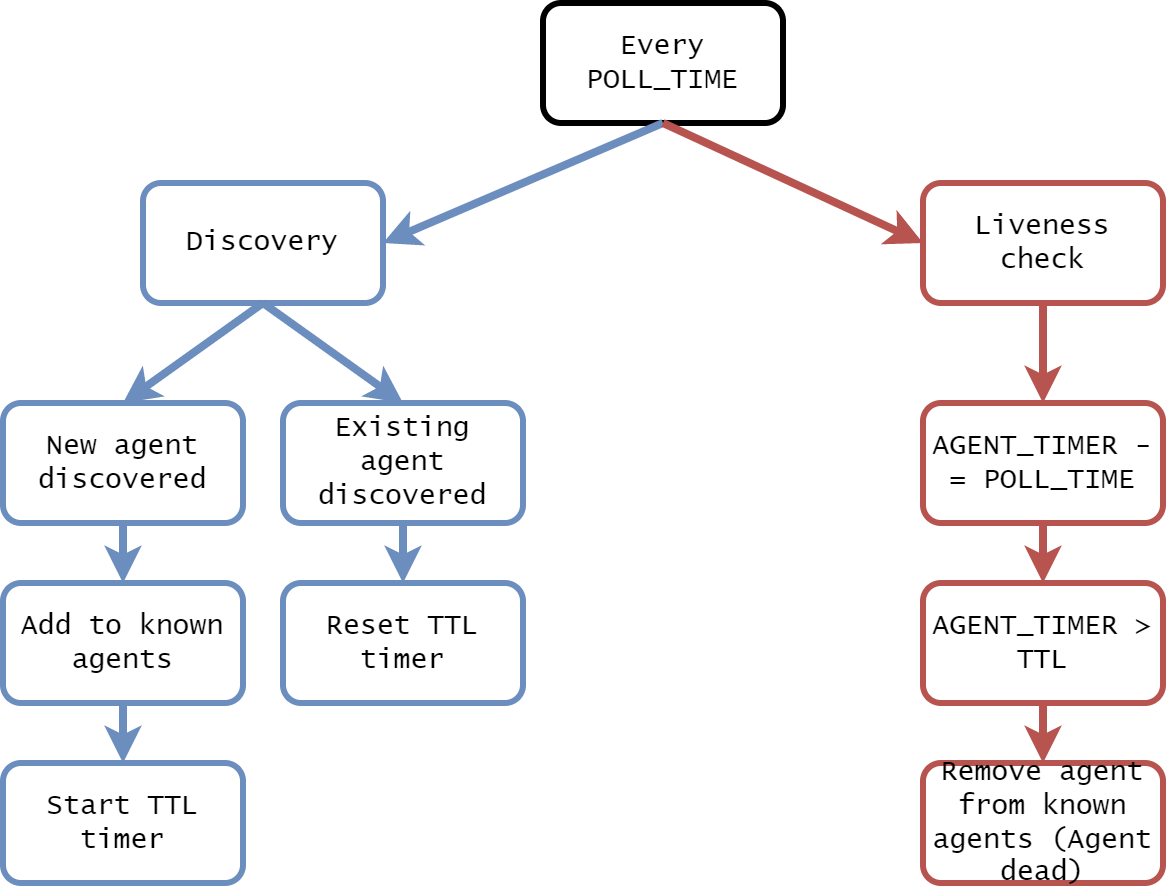
\includegraphics[width=0.8\textwidth]{pictures/agent_ttl.png}
    \caption{ Liveness check }
    \label{fig:liveness_check}
\end{figure}

Each agent will periodically send discovery message to a specific topic, to allow other agents to discover him as a peer, and mark him as alive. It will subscribe to the same topic as well to receive discovery messages from other agents. In case of new, unknown agent will be discovered, it will be added to known agents and assign and start a TTL(time to live) timer to it. If discovered agent is already known timer will be restarted.

After sending discovery message, agent will perform liveness check which means that it will decrement each known agent timer and check if timer exceeds TTL. In that case agent will be marked as dead, because it indicates that there were no messages from this particular agent for longer time that it is allowed.
